\documentclass[11pt]{article}

\usepackage{geometry}
\geometry{a4paper, portrait, margin=2cm}

\usepackage{helvet}
\renewcommand{\familydefault}{\sfdefault}

\usepackage{setspace}
\usepackage{indentfirst}
\usepackage{soul, color}
\usepackage{parskip}
\usepackage{lineno}
\usepackage{graphicx}
\usepackage[labelfont=bf]{caption}
\usepackage{float}

%opening

\begin{document}

	\begin{titlepage}
		
		\begin{center}

		\vspace*{4cm}
		\Huge
		\textbf{High Performance Computing Programming Excercises.}\\
		
		\vspace{6cm}		
			
		\large
		
		\textbf{Student:}\\
		David Bridgwood\\
		dmb2417@ic.ac.uk\\
		MRes - Computational Methods in Ecology and Evolution
		
		\end{center}
		
	\end{titlepage}
	
	\onehalfspacing
	\begin{flushleft}
	
	\section*{Neutral Theory Simulations}
	
		\subsection*{Question 8 - Neutral Time Series}
				
		 Species Richness was plotted for a Neutral Theory simulation with no speciation over 200 generations fig.\ref{fig1}. There was an initial dramatic decrease in species richness in the earlier (first 25) generations and then a more gradual decrease until the species richness eventually reached one. This will always occur where there is no speciation as at each neutral step one individual dies and is replaced by the offspring of another, as no new species are created through speciation then eventually the system will always homogenise to a species richness of one. 
		
			\begin{figure}[H]
				\centering
				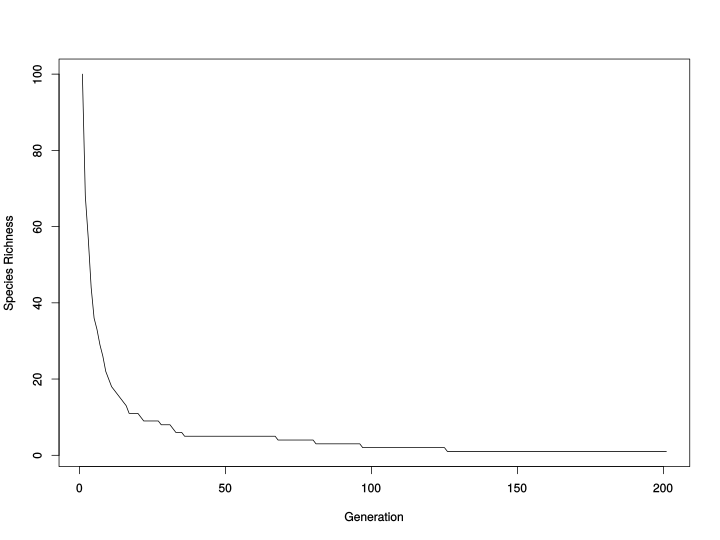
\includegraphics[width = 14.3cm]{../Results/question_8.pdf}
				\caption{Species richness moving to one when under Neutral Theory simulation with no speciation. Community Size: 100, run for 200 generations.}
				\label{fig1}
			\end{figure}
				
			
		
		\subsection*{Question 12 - Neutral Time Series with Speciation}
		
        Species Richness was plotted for a Neutral Theory simulation with a speciation rate of 0.1 and community size of 100 for 200 generations fig.\ref{fig2}, beginning at both the maximum and minimum possible species richness'. Both initial conditions reached the same dynamic equilibria for species richness. This is because now at each neutral step there are two possible outcomes, either as before one individual dies and is replaced by the identical of another, or, there is a chance (dictated by the speciation rate) that the dying individual will be replaced by an individual from a new unique species. Given that the chance of these possibilities is identical for individuals in both simulations the dynamic equilibria they reach will be the same. 

		
			\begin{figure}[H]
				\begin{center}
					\centering
				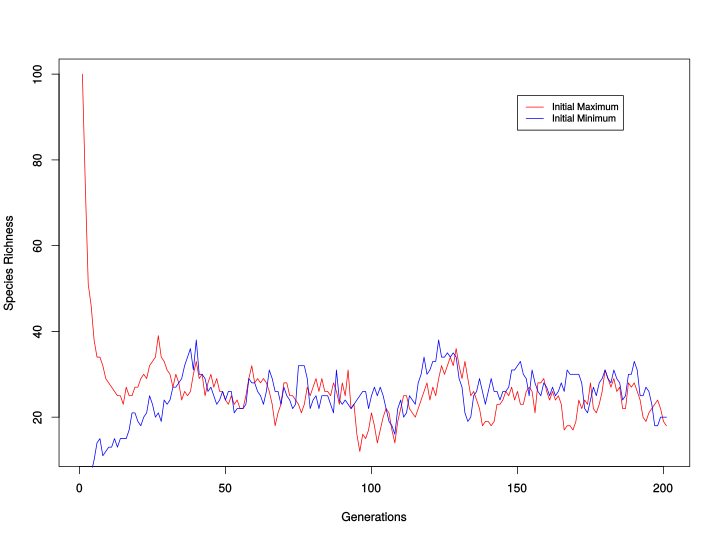
\includegraphics[width = 14.3cm]{../Results/question_12.pdf}
				\caption{Species richness under Neutral Theory simulation with 0.1 probability of speciation. Community Size: 100, run for 200 generations.}
				\label{fig2}
				\end{center}
			\end{figure}
			
			
		\subsection*{Question 16 - Species Abundances after Neutral Theory Simulation}
		
		A Neutral Theory Simulation with a speciation rate of 0.1 and community size of 100 was run for 2000 generations with an additional 200 'burn-in generations' at the start of the simulation to ensure that the simulated community had reached equilibrium before any data was recorded. After this burn-in period species abundances were recorded every 20 generations and grouped in octaves ($2^n$ to $2^n-1$). The average number of species in these octaves is shown below fig.\ref{fig3}. 
		
		As the burn-in generations are not included in the recorded species abundances the initial conditions of the community do not matter. This is because species richness quickly reaches the same equilibrium given minimum or maximum starting richness, as was shown in question 12 fig.\ref{fig2}. 
		
		
			\begin{figure}[H]
				\centering
				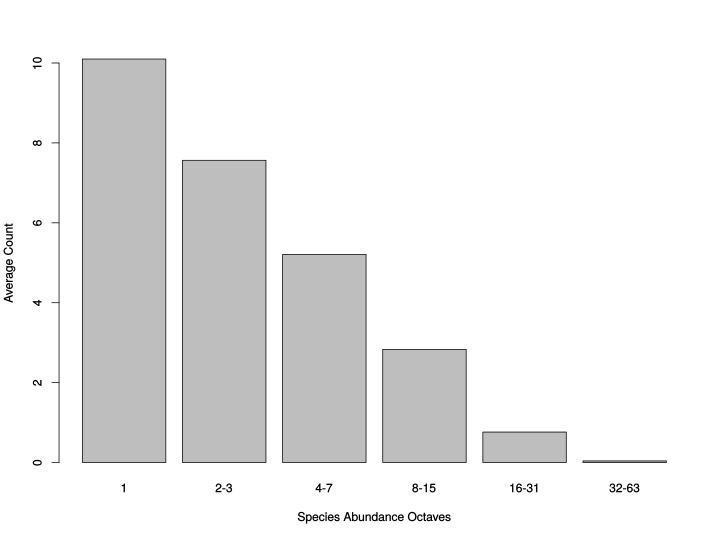
\includegraphics[width = 14.3cm]{../Results/question_16.pdf}
				\caption{Distribution of Species Abundance after a Neutral Theory Simulation with speciation rate 0.1 and community size 100, run for 2000 generations.}
				\label{fig3}
			\end{figure}
			
			
		\subsection*{Challenge Question A}
			
	     A Neutral Theory Simulation with a speciation rate of 0.1 and community size of 100 was run for 1000 generations, the species richness of the community was recorded at each iteration of the simulation (every generation). This simulation was repeated 100 times for both at initial maximum and initial minimum starting richness as the starting community. The mean species richness was plotted against generations with 97.2\% confidence limits fig.\ref{ca}. From this it is clear that the community reached dynamic equilibrium by approximately generation 50, and therefore a much shorter burn in period could have been used in question 16.
		
		
			\begin{figure}[H]
				\centering
				\includegraphics[width = 16cm]{../Results/challenge_A.pdf}
				\caption{Average species richness from 100 repeated simulations for the first 1000 generations. Community size of 100 starting at both maximum and minimum initial richness and a speciation rate of 0.1. 97.2\% confidence intervals shown. Vertical line at generation 50 - approximately where dynamic equilibrium is reached.}
				\label{ca}
			\end{figure}
			
		\subsection*{Challenge Question B}
		
		%no need for any writing!!
			
			\begin{figure}[H]
				\centering
				\includegraphics[width = \textwidth]{../Results/challenge_B.pdf}
				\caption{Average species richness from 25 repeated simulations for the first 500 generations. Community size of 100 with 11 different starting initial richness' and speciation rate of 0.1, 97.2\% confidence intervals shown.}
				\label{cb}
			\end{figure}
		

				
	\section*{Simulations Using HPC}
	
		\subsection*{Question 20 - Results from run on the Cluster}
		
		Neutral theory simulations were run on a high performance computer cluster for communities of size 500, 1000, 2500 and 5000 with a speciation rate of 0.004346. Each community size was run 25 times for 11.5 hours each simulation, with burn-in generations set to eight times the community size and species abundances recorded in octaves at regular intervals (every community size divided by 10 generations). Fig.\ref{fig4} shows the average count of these abundance octaves from all simulations for each community size and table.\ref{tbl1} provides the corresponding values.
		
			\begin{figure}[H]
				\centering
				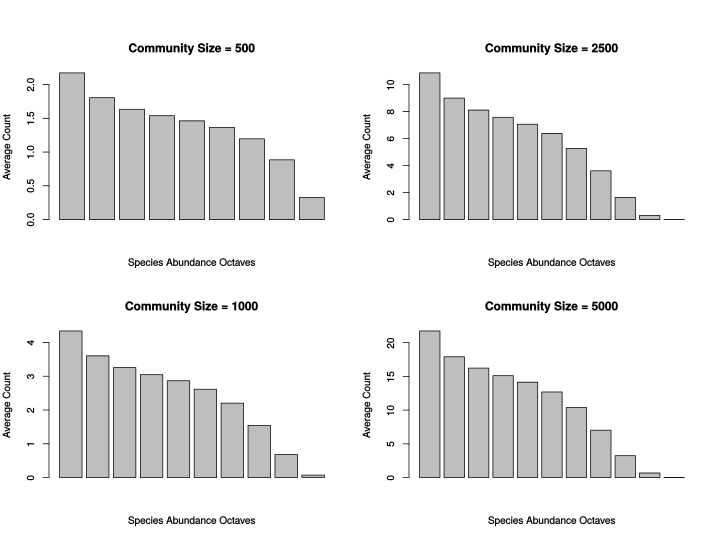
\includegraphics[width = \textwidth]{../Results/cluster_read.pdf}
				\caption{Distribution of mean Species Abundance's, shown in octaves after Neutral Theory simulations with speciation run on four different community sizes (speciation rate = 0.004346).}
				\label{fig4}
			\end{figure}
					
			\begin{table}[ht]
				\caption{Average number of species in each abundance octave (speciation rate = 0.004346).}
				\footnotesize
				\begin{tabular}{c | c c c c c c c c c c c} % centered columns (4 columns)
					\hline
					& 1 & 2-3 & 4-7 & 8-15 & 16-31 & 32-63 & 64-127 & 128-255 & 256-511 & 512-1023 & 1024-2047\\ [0.5ex]
					\hline % inserts single horizontal line
					500 & 2.173 & 1.806 & 1.634 & 1.539 & 1.463 & 1.366 & 1.196 & 0.885 & 0.327 & - & - \\
					1000 & 4.341 & 3.603 & 3.255 & 3.046 & 2.867 & 2.615 & 2.203 & 1.546 & 0.684 & 0.074 & - \\
					2500 & 10.86 & 9.002 & 8.114 & 7.578 & 7.064 & 6.374 & 5.27 & 3.608 & 1.645 & 0.309 & 0.007 \\
					5000 & 21.73 & 17.90 & 16.23 & 15.10 & 14.14 & 12.69 & 10.38 & 7.026 & 3.246 & 0.679 & 0.032 \\
					\hline %inserts single line
				\end{tabular}
				\label{tbl1}
			\end{table}
			
		\subsection*{Challenge Question C - Species Richness by Generation}
		
		Species richness reached an equilibrium after much fewer generations than were allowed in the simulation fig.\ref{fig5}. As can be seen equilibria appears to be reached at around two times the community size generations, even using a conservative four times the community size for burn in generations would have allowed for significantly more computer time to collect useful data.
		
			\begin{figure}[H]
				\centering
				\includegraphics[width = \textwidth]{../Results/challenge_C.pdf}
				\caption{Average species richness for the burn in period of each community size.}
				\label{fig5}
			\end{figure}
			
			
		\subsection*{Challenge Question D - Coalescence}
		
		Faster simulations can be performed using coalescence, as demonstrated in the function question\_d(). These simulations are much faster as they do not require a burn-in period. They also work backwards in time and strip the populations down to their speciation events meaning that a large amount of redundant simulation is not carried out - saving significant computer time.
		
					
	\newpage
	\section*{Fractals in Nature}
	
		\subsection*{Question 18 - Fractal Dimensions}
		
		The fractal dimensions of the first image shown (Sierpinski Carpet) is $(\log{(8)}/\log{(3)})$ which is approximately 1.893. This is calculated as the shape has a width of 3 and a size of 8 (8 of the original shape are required to assemble a new level of the fractal). Given that $width = size^{dimension}$, the dimension can therefore be calculated by rearranging to $dimension = \log{(size)}/\log{(width)}$.
		
		Calculated in a similar way the dimensions of the second image (Menger Sponge) is $(\log{(20)}/\log{(3)})$ approximately 2.727. As the width of the shape is still 3 but now 20 units are required to construct the next level.
		
		\subsection*{Question 19 - The Chaos Game (Sierpinski Triangle)}
		
		A Sierpinski Triangle was drawn by randomly selecting one of three points and then plotting at the mid-point between that and the current point, this was repeated 1000 times to produce the triangle below fig.\ref{fig6}.
		 
			\begin{figure}[H]
				\centering
				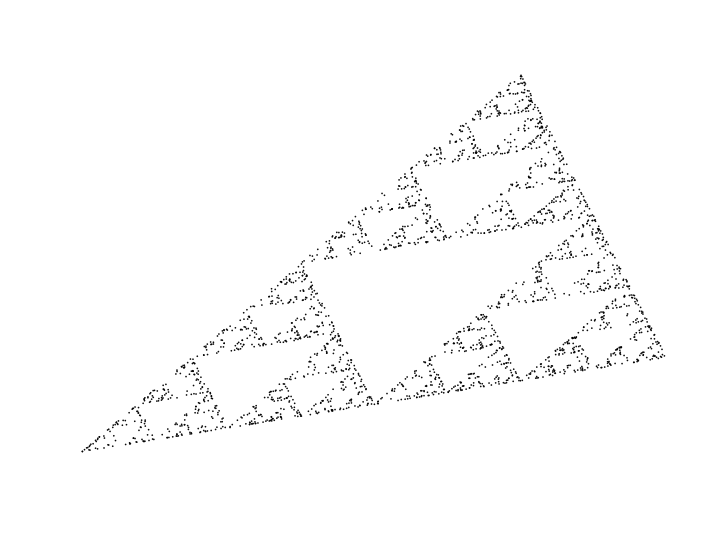
\includegraphics[width = 10cm]{../Results/chaos_game.pdf}
				\caption{Sierpinski Triangle drawn between the points: (0,0), (3,4) and (4,1).}
				\label{fig6}
			\end{figure}
					
		
		\subsection*{Challenge Question E (Sierpinski Gasket)}
		
        This Sierpinski Gasket was drawn between specific equidistant points to ensure it was an equilateral triangle fig.\ref{fig7}. The initial point was started outside of the triangle (coloured red in the top left corner), the following 20 points are also coloured red and if you look  closely you can see that a few points lie outside the triangle or within the white space but once one is plotted in the Sierpinski Gasket then all following points will also. 
		
			\begin{figure}[H]
				\centering
				\includegraphics[width = 8.5cm]{../Results/challenge_E.pdf}
				\caption{Sierpinski Gasket drawn between the points: (0,0), (4,0) and (2,$\sqrt{12}$) to make an equilateral triangle.}
				\label{fig7}
			\end{figure}
					
			
		\subsection*{Question 22 \& 23 - Spiral}
		
	   When attempting to draw a spiral a recursive function was used in R. This function called itself to continually draw lines in the direction  $\pi/4$ radians to the right and 0.95 the previous length. However this produces a stack overflow error as the computer does not know when to stop drawing lines and continually attempts to add smaller and smaller lines Ad infinitum, stopping only when it runs out of available memory.
	   
	   To overcome this problem an 'if statement' was put within the function so new lines were not drawn below a threshold length. This prevented the computer running out of memory and running into an error allowing fig.\ref{fig8} to be drawn. 
		
		
			\begin{figure}[H]
				\centering
				
\includegraphics[width = 8cm]{../Results/spiral_2.pdf}
				\caption{Spiral drawn by adding lines at $\pi/4$ radians to the right and 0.95 length until new lines went below a threshold length.}
				\label{fig8}
			\end{figure}
		
			
		\subsection*{Question 24 - Tree}
		
		 Similar to the spiral function, the tree function calls itself but this time twice, once with a direction of $pi/4$ radians to the right and once the same to the left. The length also decreases more at each iteration, this time 0.65 times. The function produces the below fractal tree fig.\ref{fig9}.
		
			\begin{figure}[H]
				\centering
				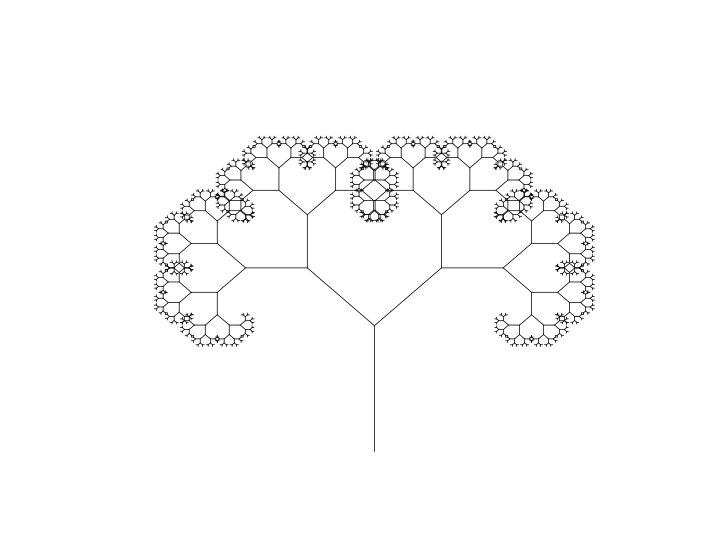
\includegraphics[width = 14.3cm]{../Results/tree.pdf}
				\caption{Tree drawn by calling itself twice in the same function with direction $\pi/4$ radians to the right and to the left.}
				\label{fig9}
			\end{figure}
			
			
		\subsection*{Quesiton 26 - Fern\_2}
		
	    A modified version of the tree function again calls itself twice, once with direction $pi/4$ radians and once straight up. An additional variable was added to dictate if the new branch should go to the left or the right and the function was written in such a way to alternate between the two possibilities. The resulting image is shown in fig.\ref{fig10}. 
	
			\begin{figure}[H]
				\centering
				\includegraphics[width = 14.3cm]{../Results/fern_2.pdf}
				\caption{Fern drawn by modifying the tree function to alternate the direction of branches.}
				\label{fig10}
			\end{figure}
			
			
		\subsection*{Challenge Question F}
		
	        Changing the minimum threshold length below which the computer stopped adding branches had a significant impact on the time it took for the fern\_2 function to run. With an initial length of 1 it took my (not particularly powerful) computer 0.169s to draw a fern when this threshold value was set to 0.1, changing this value to 0.005 had a significant impact on the time taken - now 23.599s. This is due to the fact that with each new iteration the computer has to draw exponentially more lines - two for each previous line drawn.  
		
			\subsubsection*{Challenge\_F1}
			
            By modifying the fern\_2 function I was able to produce an image of a Christmas tree fig.\ref{fig11}. Now the branches alternate between going directly up or down, I made the branches a little thicker and longer so there was some overlap so the tree looked more densely packed. Each lines colour is randomly sampled from a list of different shades of green which hopefully adds to the realism. 
            
            I also attempted to write a function for a Koch Snowflake to put at the top of the tree as a star (challenge\_F1.1), I wasn't completely successful, but you can see I was starting to get close.
			
					\begin{figure}[H]
						\centering
						\includegraphics[width = 14.3cm]{../Results/challenge_F1.pdf}
						\caption{Modified Fern to look like a Christmas tree with an attempted Koch Snowflake as a star.}
						\label{fig11}
					\end{figure}
					

	\end{flushleft}
	
\end{document}